\subsection{Willowbrook}

Willowbrook has twelve places (a café, a library, a college, a park, a pub, a town hall and others) and 25 residents with jobs, homes, weekly routines, favourite places and interests. Time advances in steps of 15 minutes. The cognitive loop follows Generative Agents, with every call to the language model replaced by a rule.
\begin{itemize}
\item \textbf{Perception.} At every step a resident observes what it is doing and what up to three other people at the same place are doing. New observations enter its memory stream with an importance that depends on the activity (sleeping 1, routine at home 2, work or leisure 3, chatting 4, attending an event 7) plus a small random offset.
\item \textbf{Conversation.} Residents at the same place talk with a probability that depends on their sociability. Before talking, the speaker retrieves memories with the focal points used by \code{converse.py} in the reference code, the listener's name ($k=50$) and ``\emph{listener} is \emph{activity}'' ($k=25$). With probability 0.5 it then passes on the most important piece of news among the retrieved memories that it has not yet exchanged with this listener, otherwise the two make small talk. Both remember the conversation.
\item \textbf{Planning.} At wake-up and at 14:00 every resident retrieves memories with the focal points of \code{plan.py}, ``\emph{name}'s plan for \emph{date}.'' and ``Important recent events for \emph{name}'s life.'' ($k=30$ each). If an event of that day is among the retrieved memories, the resident attends it with a fixed probability.
\item \textbf{News.} Every eight hours somebody learns a piece of gossip (a new puppy, a promotion, a picnic on Thursday). The scenario of the paper is reproduced on top of this: Maria Lopez, who runs the café, learns 35 hours in advance that she is hosting a party there at 5 pm. She invites everyone she talks to.
\end{itemize}
Every retrieval refreshes the access time of the memories it returns. Random decisions use counter-based hashing, so two runs with the same seed see the same world and diverge only where their retrievals differ.

\textbf{Calibration.} Two parameters have no counterpart in the paper, the conversation rate and the probability of passing on news. They were chosen with exact retrieval in a young town (two days of memories) so that the outcome matches the Valentine's Day party of \citet{park2023generative}, where 13 of the 25 agents knew about the party after two game days and 5 of the 12 invited agents came. Over a grid of 15 settings with 12 seeds each (\code{experiments/calibrate\_town.py}), a conversation rate of 0.06 and a sharing probability of 0.5 give \CalKnew{} knowing agents and \CalAttended{} guests on average.

\textbf{Experiment.} The independent variable is the age of the town when Maria learns about the party: 2 days, as in the paper, or 9, 32 or 92 days, so that every agent carries a larger memory into the scenario. Each age was run with 30 seeds and four retrieval methods, all with the paper's score (min-max, $a=b=c=1$): the exact scan, the folded store, overfetch with $K=100$ and relevance only. The outcomes are the number of agents who knew about the party before it started, who had it among their retrieved memories when planning the day and who attended.

\subsection{Results}

\Cref{fig:town,tab:town} show the outcomes. In a young town the four methods agree: with about a hundred memories per agent, the party ranks high under any of them. From nine days on they drift apart, because the approximate methods return a shrinking share of the paper's top-$k$ as the memories grow: after three months, \TNinetyReRecall{} for overfetch and \TNinetyRelRecall{} for relevance only (\cref{fig:garecency}, right).

\textbf{The folded store behaves like the exact scan.} Its retrievals contain \TNinetyFoRecall{} of the paper's top-$k$ after 92 days. The three outcomes are identical on every seed up to 32 days and on \TNinetyFoSame{} of the \TNinetySeeds{} seeds at 92 days. On the other seeds they differ by at most \TNinetyFoMaxDiff{} agents, in both directions.

\textbf{Relevance-only memory loses about 40\% of the diffusion.} From nine days on, \TRelDropAwareLo{} to \TRelDropAwareHi{} fewer agents know about the party and \TRelDropAttLo{} to \TRelDropAttHi{} fewer attend it (\TNinetyRelAware{} against \TNinetyExAware{} knowing agents and \TNinetyRelAtt{} against \TNinetyExAtt{} guests at 92 days). The invitation travels through conversations. The focal point of a conversation is the listener's name, which the party is rarely similar to. Without recency and importance the agents do not think of mentioning it.

\textbf{Overfetch and re-rank moves the outcome in both directions.} At 9 and 32 days it spreads the news slightly less than the exact scan (\TThirtyReAware{} against \TThirtyExAware{} knowing agents at 32 days). At 92 days it spreads it clearly more: \TNinetyReAware{} agents know about the party and \TNinetyReRecalled{} recall it when planning, against \TNinetyExAware{} and \TNinetyExRecalled{}, although it returns less than half of the paper's top-$k$. The reason is the second half of its candidate set, the newest memories. A piece of news is among an agent's newest memories right after it is heard, so it always becomes a candidate, while most of the recent observations that would outrank it under the full score are neither that new nor similar enough to the focal point and never reach the re-ranking. Taking the newest memories out of the candidate set confirms this. With only the 100 most similar memories, the outcome at 92 days falls to \TNinetyNrAware{} knowing agents and \TNinetyNrAtt{} guests (\TThirtyNrAware{} and \TThirtyNrAtt{} at 32 days), close to relevance-only memory, although the share of the paper's top-$k$ it retrieves hardly changes (\TNinetyNrRecall{} against \TNinetyReRecall{}).

Two conclusions follow. An approximate retrieval does not lose information at random: it changes which information the agents act on. The direction of the change depends on details such as which recent memories enter the candidate set and how large the memory has grown. And recall against the paper's top-$k$ does not predict the effect, since two methods with the same recall led the town to very different outcomes.

\begin{figure}[t]
\centering
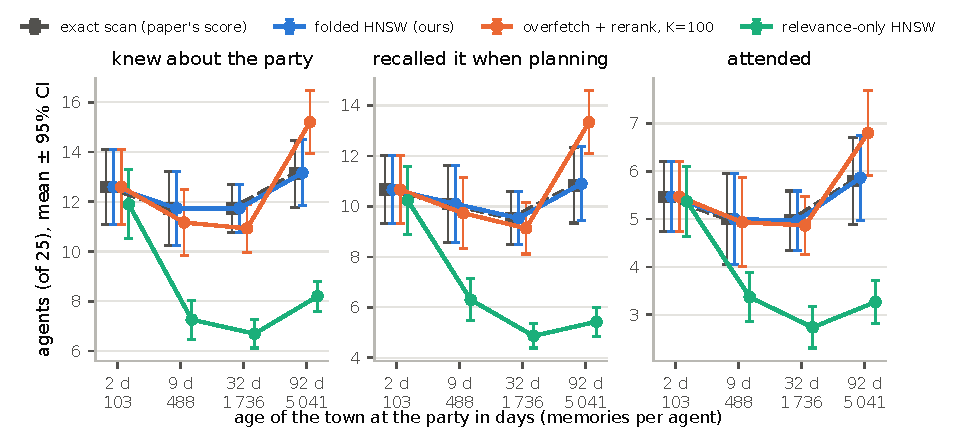
\includegraphics[width=0.99\linewidth]{town_outcomes}
\caption{The party scenario in towns of increasing age (30 seeds each, mean and 95\% confidence interval). The folded store reproduces the exact scan on every seed up to 32 days and on \TNinetyFoSame{} of \TNinetySeeds{} at 92 days.}
\label{fig:town}
\end{figure}

\begin{table}[t]
\centering\small
\begin{tabular}{l l r r r r r}
\toprule
Age & Retrieval & memories & recall & knew & recalled & attended\\
\midrule
2 days & Exact scan (paper) & 103 & 1.000 & 12.6 $\pm$ 1.5 & 10.7 $\pm$ 1.3 & 5.5 $\pm$ 0.7\\
 & Folded HNSW (ours) & 103 & 1.000 & 12.6 $\pm$ 1.5 & 10.7 $\pm$ 1.3 & 5.5 $\pm$ 0.7\\
 & Overfetch + re-rank, $K{=}100$ & 103 & 0.995 & 12.6 $\pm$ 1.5 & 10.7 $\pm$ 1.3 & 5.5 $\pm$ 0.7\\
 & Relevance only & 103 & 0.872 & 11.9 $\pm$ 1.4$^{**}$ & 10.2 $\pm$ 1.3$^{**}$ & 5.4 $\pm$ 0.7\\
\addlinespace
9 days & Exact scan (paper) & 488 & 1.000 & 11.7 $\pm$ 1.5 & 10.1 $\pm$ 1.5 & 5.0 $\pm$ 1.0\\
 & Folded HNSW (ours) & 488 & 1.000 & 11.7 $\pm$ 1.5 & 10.1 $\pm$ 1.5 & 5.0 $\pm$ 1.0\\
 & Overfetch + re-rank, $K{=}100$ & 487 & 0.876 & 11.2 $\pm$ 1.3$^{**}$ & 9.7 $\pm$ 1.4$^{*}$ & 4.9 $\pm$ 0.9\\
 & Relevance only & 484 & 0.637 & 7.3 $\pm$ 0.8$^{**}$ & 6.3 $\pm$ 0.8$^{**}$ & 3.4 $\pm$ 0.5$^{**}$\\
\addlinespace
32 days & Exact scan (paper) & 1736 & 1.000 & 11.7 $\pm$ 1.0 & 9.5 $\pm$ 1.0 & 5.0 $\pm$ 0.6\\
 & Folded HNSW (ours) & 1736 & 1.000 & 11.7 $\pm$ 1.0 & 9.5 $\pm$ 1.0 & 5.0 $\pm$ 0.6\\
 & Overfetch + re-rank, $K{=}100$ & 1734 & 0.681 & 10.9 $\pm$ 1.0$^{*}$ & 9.1 $\pm$ 1.0$^{*}$ & 4.9 $\pm$ 0.6\\
 & Relevance only & 1725 & 0.488 & 6.7 $\pm$ 0.6$^{**}$ & 4.9 $\pm$ 0.5$^{**}$ & 2.7 $\pm$ 0.4$^{**}$\\
\addlinespace
92 days & Exact scan (paper) & 5041 & 1.000 & 13.1 $\pm$ 1.3 & 10.8 $\pm$ 1.5 & 5.8 $\pm$ 0.9\\
 & Folded HNSW (ours) & 5041 & 0.999 & 13.2 $\pm$ 1.3 & 10.9 $\pm$ 1.5 & 5.9 $\pm$ 0.9\\
 & Overfetch + re-rank, $K{=}100$ & 5034 & 0.487 & 15.2 $\pm$ 1.3$^{**}$ & 13.3 $\pm$ 1.3$^{**}$ & 6.8 $\pm$ 0.9$^{*}$\\
 & Relevance only & 5007 & 0.366 & 8.2 $\pm$ 0.6$^{**}$ & 5.4 $\pm$ 0.6$^{**}$ & 3.3 $\pm$ 0.5$^{**}$\\
\bottomrule
\end{tabular}

\caption{The party scenario by age of the town. Memories per agent at the end of the run, mean recall of the paper's top-$k$ over all retrievals and the number of agents (of 25) who knew about the party, recalled it when planning and attended, as mean $\pm$ 95\% confidence interval over 30 seeds. Stars mark a difference from the exact scan in a paired Wilcoxon test ($^{*}p<0.05$, $^{**}p<0.01$).}
\label{tab:town}
\end{table}
